	\section{Рангирање страница}
	Пошто је завршен к\^{о}д \emph{crawl\_web} процедуре и када постоји веб-паук који може на задовољавајући начин да скенира странице, смешта линкове у индекс или хеш табелу и да даје резултате у односу на постављене упите, следећи корак је рангирање страница. Рангирање страница је и најзахтевнији део веб претраживача. На почетку поглавља је поменут алгоритам за рангирање страница \emph{PageRank}$^tm$\index{PageRank@\emph{PageRank}}, који је срце Гугловог претраживача. У оквиру овог рада реализоваће се алгоритам сличан \emph{PageRank}$^tm$ алгоритму у Python програмском језику. 
		\subsection{Такмичење у популарности}
		Поставља се питање: ко је популаран? Шта је популарност\index{PageRank@\emph{PageRank}!popularnost@популарност}? Ако Ана има највише пријатеља да ли је она најпопуларнија? У школи, на пример, није најважније имати пуно пријатеља, поготово ако су ти пријатељи особе које немају много пријатеља. Важно је и да пријатељи буду популарни. Такође, треба имати у виду и да особа која има јако пуно пријатеља то пријатељство баш и не цени, те тиме и популарност опада.\\
		Теза оснивача Гугла, Брина и Пејџа, каже\cite[Ch 4]{langville2011google} \begin{quote}
		\textit{Страница је важна ако се на њу показује са других важних страница.}
		\end{quote}
		Прва верзија формуле за израчунавање популарности у PageRank алгоритму је сличила следећем:
		\begin{equation}\label{eq:rank1}
		rank(P_{i})=\sum_{P_{j}\in B_{P_{i}}}\frac{rank(P_{j})}{\left |P_{j}  \right |}
		\end{equation}
		где је $P_{i}$ $i$-та страница, $B_{P_{j}}$ скуп страна које показују на $P_{ј}$, $\left |P_{j}  \right |$ број излазних линкова од $P_{j}$. Проблем са формулом \ref{eq:rank1} је у томе што не може да се одреди број $P_{j}$, одн. број линкова од $P_{j}$ ка $P_{i}$. Проблем је решен коришћењем итеративне методе. Дакле, у почетку све странице имају ранг $\frac{1}{n}$, где је $n$, број страница у Гугловом индексу. Тако да се сада рачуна сваки $rank(P_{i})$ за сваку страницу $P_{i}$ из индекса и онда само треба одредити после колико итерација $k$ ће $rank_{k+1}(P_{i})$ бити довољно прецизан. Тако да формула гласи\cite[Ch 4.1]{langville2011google}
		\begin{equation}\label{eq:rank2}
		rank_{k+1}(P_{i})=\sum_{P_{j}\in B_{P{j}}}\frac{rank_{k}(P_{j})}{\left |P_{j}  \right |}
		\end{equation}
		где је $rank_{0}(P_{i})=\frac{1}{n}$ за сваку страницу из индекса.\\
		На пример, ако се претпостави да постоји овакав оријентисан граф\index{graf@граф} на слици \ref{slike:graf}, који представља модел четири веб странице, где су хипервезе представљане уређеним везама. 
		\begin{figure}[here]
		\centering
		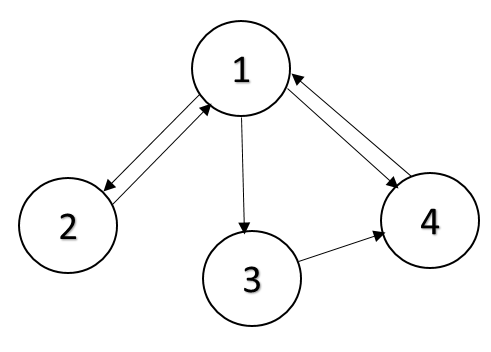
\includegraphics[scale=0.6]{graf.png}
		\caption{Оријентисани граф модела четири веб странице}
		\label{slike:graf}
		\end{figure}
		
		Израчунавање ранга\index{PageRank@\emph{PageRank}!rang@ранг} у две итерације је представљано у табели \ref{tabele:rank}.
		\begin{table}[h]
		
		\centering
		\def\arraystretch{1.5}
		\begin{tabular}{|c|c|c|c|}\hline
		\textbf{итерација 0} & \textbf{итерација 1} & \textbf{итерација 1} & \textbf{PageRank}\\ \hline\hline
		$rank(1)=\frac{1}{4}$ & $\frac{1}{2}$ & $\frac{5}{12}$ & \textrm{I} \\ \hline
		$rank(2)=\frac{1}{4}$ & $\frac{1}{12}$ & $\frac{1}{6}$ & \textrm{III} \\ \hline
		$rank(3)=\frac{1}{4}$ & $\frac{1}{12}$ & $\frac{1}{6}$ & \textrm{III} \\ \hline
		$rank(4)=\frac{1}{4}$ & $\frac{1}{3}$ & $\frac{1}{4}$ &  \textrm{II}\\ \hline
		\end{tabular}
		
		\caption{Израчунавање PageRank-а у две итерације}
		\label{tabele:rank}
        \end{table}		
        \pagebreak
        \subsection{Матрични облик} 
		Аутори  PageRank-а су заменили суму вектором и од вектора направили матрични модел. Нека је $H$ матрица\index{PageRank@\emph{PageRank}!matrica@матрица} димензија $m\times n$, таква да је $H_{ij}=\frac{1}{\left |P_{i}  \right |}$, ако постоји линк од $i$ ка $j$ или $0$ у супротном. Тада би матрица графа била: 
\[
H=
\begin{blockarray}{ccccc}
& 1 & 2 & 3 & 4  \\
\begin{block}{c(cccc)}
  1 & 0 & \frac{\strut 1}{\strut 3} & \frac{\strut 1}{\strut 3} & \frac{\strut 1}{\strut 3}  \\
  2 & 1 & 0 & 0 & 0  \\
  3 & 0 & 0 & 0 & 1  \\
  4 & 1 & 0 & 0 & 0  \\
\end{block}
\end{blockarray}
 \]
        Нека је $\pi^{T}$ вектор, такав $\pi^{(k)T}$ представља PageRank вектор\index{PageRank@\emph{PageRank}!vektor@вектор} у итерацији $k$. Тада се следећа итерација добија као:
        \begin{equation}
        \pi^{(k+1) T}=\pi^{(k)T}H
        \end{equation}
        Свака итерација захтева једно множење вектора и матрице, што нам даје $O(n^{2})$ израчунавања. Но, како је матрица $H$ са врло мало не-нула поља, она захтева $O(nnz(H))$ израчунавања, где је $nnz(H)$ број ненула елемената матрице $H$. Такође, матрица $H$ веома личи на транзициону стохастичку матрицу\index{Markovljevi lanci@Марковљеви ланци!stohasticka matrica@стохастичка матрица} Марковљевих ланаца\index{Markovljevi lanci@Марковљеви ланци}\footnote{Марковљеви ланци описују стохастичке системе(\emph{стохастичке или вероватносне}, прим. аут.) "без меморије", тј. такве системе код којих вероватноће будућих стања зависе само од садашњег, а не од прошлих стања.\cite{filipovic2006operatori}} тако да је можемо назвати субстохастичком\cite[Ch 4.2]{langville2011google}. Брин и Пејџ нису користили термин "Марковљев ланац". Али оно што јесу урадили је да су матрицу $H$ врло мало модификовали како би она била стохастичка. Уместо термина "Марковљев ланац"\index{Markovljevi lanci@Марковљеви ланци}, користили су термин "случајни сурфер"(енгл. \emph{random surfer})\index{PageRank@\emph{PageRank}!random surfer@\emph{random surfer}}. Када такав сурфер дође на страницу са неколико хипервеза, он бира једну од њих на случајан начин и наставља тај процес унедоглед. У дужем временском периоду, део времена који сурфер\index{PageRank@\emph{PageRank}!random surfer@\emph{random surfer}} проводи на датој веб страници је мерило о релативној важности те странице. Ако он проводи доста времена на некој страници, онда мора да се стално враћа на ту страну. Странице које он поново посећује морају бити важне зато што на њих показују друге важне странице.\\
        Два су главна проблема са иницијалним \emph{случајним сурфером}:
        \begin{description}
        \item[dangling node] овај термин означава чвор графа који не показује ни на један други чвор
        \item[конвергенција] да ли ће и после колико итерације, алгоритам дати исправне и очекиване резултате
        \end{description}
        Као резултат решавања првог проблема, добија се модификована матрица која решава тај проблем, уз помоћ :
        \begin{equation}
        S = H + a(\frac{1}{n}e^{T})
        \end{equation}
        где је $e^T$ јединични вектор, а $a = \left\{\begin{matrix}
1, & dangling\; node \\ 
0, & inace
\end{matrix}\right.$ и $n$ остаје број страница у индексу.\\
        Други проблем, тј. проблем конвергенције, је решен тиме што се матрица $S$ модификовала тако да она постане стохастичка, несводљива, апериодична и примитивна, те тако и конвергира. Модификација матрице $S$ ради се у неколико корака: 
        \begin{equation}
        G = \alpha S + (1-\alpha)\frac{1}{n}ee^{T}
        \end{equation}
        \begin{equation}
        G = \alpha(H + a(\frac{1}{n}e^{T})+(1-\alpha)\frac{1}{n}ee^{T}
        \end{equation}
        \begin{equation}
        G = \alpha H + (\alpha a + (1-\alpha)e)\frac{1}{n}e^{T}
        \end{equation}
        где је $0\leqslant\alpha\leqslant1$ параметар који даје својство \emph{телепортације} случајном сурферу\index{PageRank@\emph{PageRank}!random surfer@\emph{random surfer}}, тј могућност да почне процес из почетка. На пример ако је $\alpha=0.6$ то значи да ће 60\% времена случајни сурфер проводити време кликћући линкове, а 40\% времена ће почињати процес из почетка, бирајући случајним одабиром нову страницу за почетак.\\
        У примеру са слике \ref{slike:graf} после краћег рачунања добија се следећа матрица $G$:
\[G = 
\begin{bmatrix}
0.025 & 0.325 & 0.325 & 0.325 \\ 
0.925 & 0.025 & 0.025 & 0.025 \\ 
0.025 & 0.025 & 0.025 & 0.925 \\ 
0.925 & 0.025 & 0.025 & 0.025
\end{bmatrix}
\]
\pagebreak
       \subsection{Израчунавање вредности PageRank\texttrademark{} вектора}
       Вектор $\pi^{T}$\index{PageRank@\emph{PageRank}!vektor@вектор} је могуће добити на два начина, уз услов да је $\pi^{T}e = 1$:
       \begin{enumerate}
       \item Налажењем леве сопствене вредности матрице\index{sopstvene vrednosti matrice@сопствене вредности матрице} $G$, тј $\pi^{T}G=\lambda \pi^{T}$
       \item Налажењем левог нула вектора од $I - G$, тј. $\pi^{T}(I-G)=O^{T}$
       \end{enumerate}
       У примеру са слике \ref{slike:graf} добија се: $\pi^{T} = \left [0.7608\: 0.2740\: 0.2740\: 0.5206 \right ]$\footnote{Израчунато у Python-у, помоћу модула numpy\index{numpy@\emph{numpy}} - \texttt{www.numpy.org} и scypy\index{scypy@\emph{scypy}} \texttt{www.scypy.org}} 
       \begin{lstlisting}[caption=Израчунавање леве сопствене вредности, label={lst:eigen}, numbers=left]
import numpy as np
from scipy.linalg import eig

T = np.mat("0.025 0.325 0.325 0.325;
            0.925 0.025 0.025 0.025; 
            0.025 0.025 0.025 0.925; 
            0.925 0.025 0.025 0.025")
            
values, left = eig(T, left = True, right = False)

for i in range(len(values)):
	print("Levi sopstveni vektor za sopstvenu vrednost {}:".format(values[i]))
	print(left[:,i])
	print()
>>>Levi sopstveni vektor za sopstvenu vrednost (0.9999999999999998+0j):
[-0.76083506+0.j -0.27398492+0.j -0.27398492+0.j -0.52057136+0.j]
        \end{lstlisting}
        Тумачећи резултате, долази се до закључка да је страница \textbf{1} најпопуларнија, јер има највећу вредност, друга је страница \textbf{4}, а треће место деле странице \textbf{2} и \textbf{3}.
\pagebreak		
		\subsection{Рангирање веб страница у Python-у}
		Имплементација ове варијанте PageRank\index{PageRank@\emph{PageRank}} алгоритма у crawl\_web модул се врши додавањем још једне структуре - граф, како би се знало на који начин је случајни сурфер\index{PageRank@\emph{PageRank}!random surfer@\emph{random surfer}} прегледавао странице. Граф\index{graf@граф} ће се једноставно иницијализовати у самој функцији crawl\_web, као празна мапа. Граф би требао садржи хипервезу као кључ и листу хипервеза на које показује, као вредност. Тако да измењена функција crawl\_web изгледа овако:
		\begin{lstlisting}[caption=Увођење графа у crawl\_web, label={lst:graph}, numbers=left]
def crawl_web(seed):
    tocrawl = [seed]
    crawled = []
    graph = {}  # <url>, [lista stranica na koje pokazuje]
    index = {} 
    while tocrawl: 
        page = tocrawl.pop()
        if page not in crawled:
            content = get_page(page)
            add_page_to_index(index, page, content)
            
            outlinks = get_all_links(content)
            graph[page]=outlinks # pravljenje grafa
            
            union(tocrawl, outlinks)
            crawled.append(page)
    return index, graph
		\end{lstlisting}
		\subsection{Израчунавање ранга странице}
		Ранг\index{PageRank@\emph{PageRank}!rang@ранг} странице ће у овом раду бити израчунат помоћу формуле \ref{eq:rank2}, измењену за \emph{dumping} константу, која је позитивна и није већа од 1. Познато је и да је почетна вредност свих страница у нултом кораку итерације иста и изности $\frac{1}{n}$. Дакле,
		\begin{equation}\label{eq:zero}
		rank(0, P_{i})=\frac{1}{n}
		\end{equation}
		\begin{equation}
		rank(k+1, P_{i})=\alpha \sum_{P_{j} \in B_{P_{j}}}\frac{rank(k, P_{j})}{\left |P_{j}  \right |} + (1-\alpha)\frac{1}{n}
		\end{equation}
		Оваква поставка намеће рекурзију\index{rekurzija@рекурзија} као решење, али како није унапред познат број рачунања, тиме је опрезније применити итерацију приликом рачунања. Уз листинг кода \ref{lst:dictionary} и уз измењену функцију crawl\_web из листинга \ref{lst:graph}, сада ће се придодати и функција за израчунавање ранга странице \emph{rank\_compute}, која узима граф као улаз и враћа мапу, чија је кључна реч хипервеза, а вредност је њен ранг.
		\pagebreak
		\begin{lstlisting}[caption=Израчунавање ранга странице, label={lst:rank}, numbers=left]
def compute_ranks(graph):
    alfa = 0.9 # damping faktor
    numloops = 10 # broj iteracija
    
    ranks = {}
    npages = len(graph)
    for page in graph:
        ranks[page] = 1.0 / npages
    
    for i in range(0, numloops):
        newranks = {}
        for page in graph:
            newrank = (1 - alfa) / npages
            
            for node in graph:
                if page in graph[node]:
                    newrank += ranks[node]*alfa/len(graph[node])
            
            newranks[page] = newrank
        ranks = newranks
    return ranks
		\end{lstlisting}
		На крају остаје још да се сортирају резултати и да се омогући кориснику да страницу са највећим рангом види као прву. Ради тога се уводи функција \emph{results}, која ће узети индекс, рангове који су постављени у мапу и наравно, кључну реч корисника. Као резултат се даје листа са свим релевантним хипервезама који су поређани по рангу. 
		\begin{lstlisting}[caption=Функција која враћа најбољи резултат, label={lst:results}, numbers=left]
def results(index, ranks, keyword):
    urls = lookup(index, keyword)
    if urls == None:
        return None
    results_url = []    
    results_num = []
    for e in urls:
        results_num.append(ranks[e])
    results_num.sort()
    while results_num:
        current_max = results_num.pop()
        for url in urls:
            if ranks[url]==current_max:
                results_url.append(url)
                break
    return results_url
      
		\end{lstlisting}
		Овим је у потпуности реализован алгоритам за претраживање веба. К\^{о}д је у целости дат у Додатку А (видети поглавље \ref{sec:dodataka}).